%\documentclass[draft,10pt]{beamer}
\documentclass[10pt]{beamer}

% \usepackage{define}

\usetheme{CCFD}
\usepackage{color}
\definecolor{gray97}{gray}{.90}
\definecolor{gray75}{gray}{.75}
\usepackage{listings}
\lstset{frame=Ltb, showspaces=false,showstringspaces=false,
     framerule=0pt,
     aboveskip=0cm,
     framextopmargin=0pt,
     framexbottommargin=1pt,
     framexleftmargin=0.1cm,
     framesep=1pt,
     rulesep=.4pt,
     backgroundcolor=\color{gray97},
     rulesepcolor=\color{black},
     language=C,
           basicstyle=\ttfamily\scriptsize,
           keywordstyle=\color{blue}\ttfamily,
           stringstyle=\color{red}\ttfamily,
           commentstyle=\color{teal}\ttfamily,
          breaklines=true,
          %
          numbers=left,
          numberstyle=\tiny,
          numbersep=-5pt,
%           numberfirstline = false,
%           breaklines=true
          }
\lstdefinestyle{consol}
   {basicstyle=\scriptsize\bf\ttfamily,
    backgroundcolor=\color{gray75},
}
\resetcounteronoverlays{lstnumber}

\usepackage{tikz}
\usetikzlibrary{calc,shapes}

\eventtitle{Computer Science I}
\title{Computer Science I}
\author[shortname]{Dr. inż Nikesh}
\institute[shortinst]{room 117,\\ nikesh.yadav@pw.edu.pl}
\date{}

\setbeamertemplate{blocks}[rounded][shadow=true]
\setbeamertemplate{navigation symbols}[]

\begin{document}

\frame{
    \titlepage
}

%%%%%%%%%%%%%%%%%%%%%%%%%%%%%%%%%%%%%%%%%%%%%%%%%%%%%%%%%%%%%%%%%%%%%%%
\section{Rules and Regulations}
%%%%%%%%%%%%%%%%%%%%%%%%%%%%%%%%%%%%%%%%%%%%%%%%%%%%%%%%%%%%%%%%%%%%%%%

% \frame{
%   \frametitle{Rules and regulations}
%   \vspace{0cm}
%   \centering
%   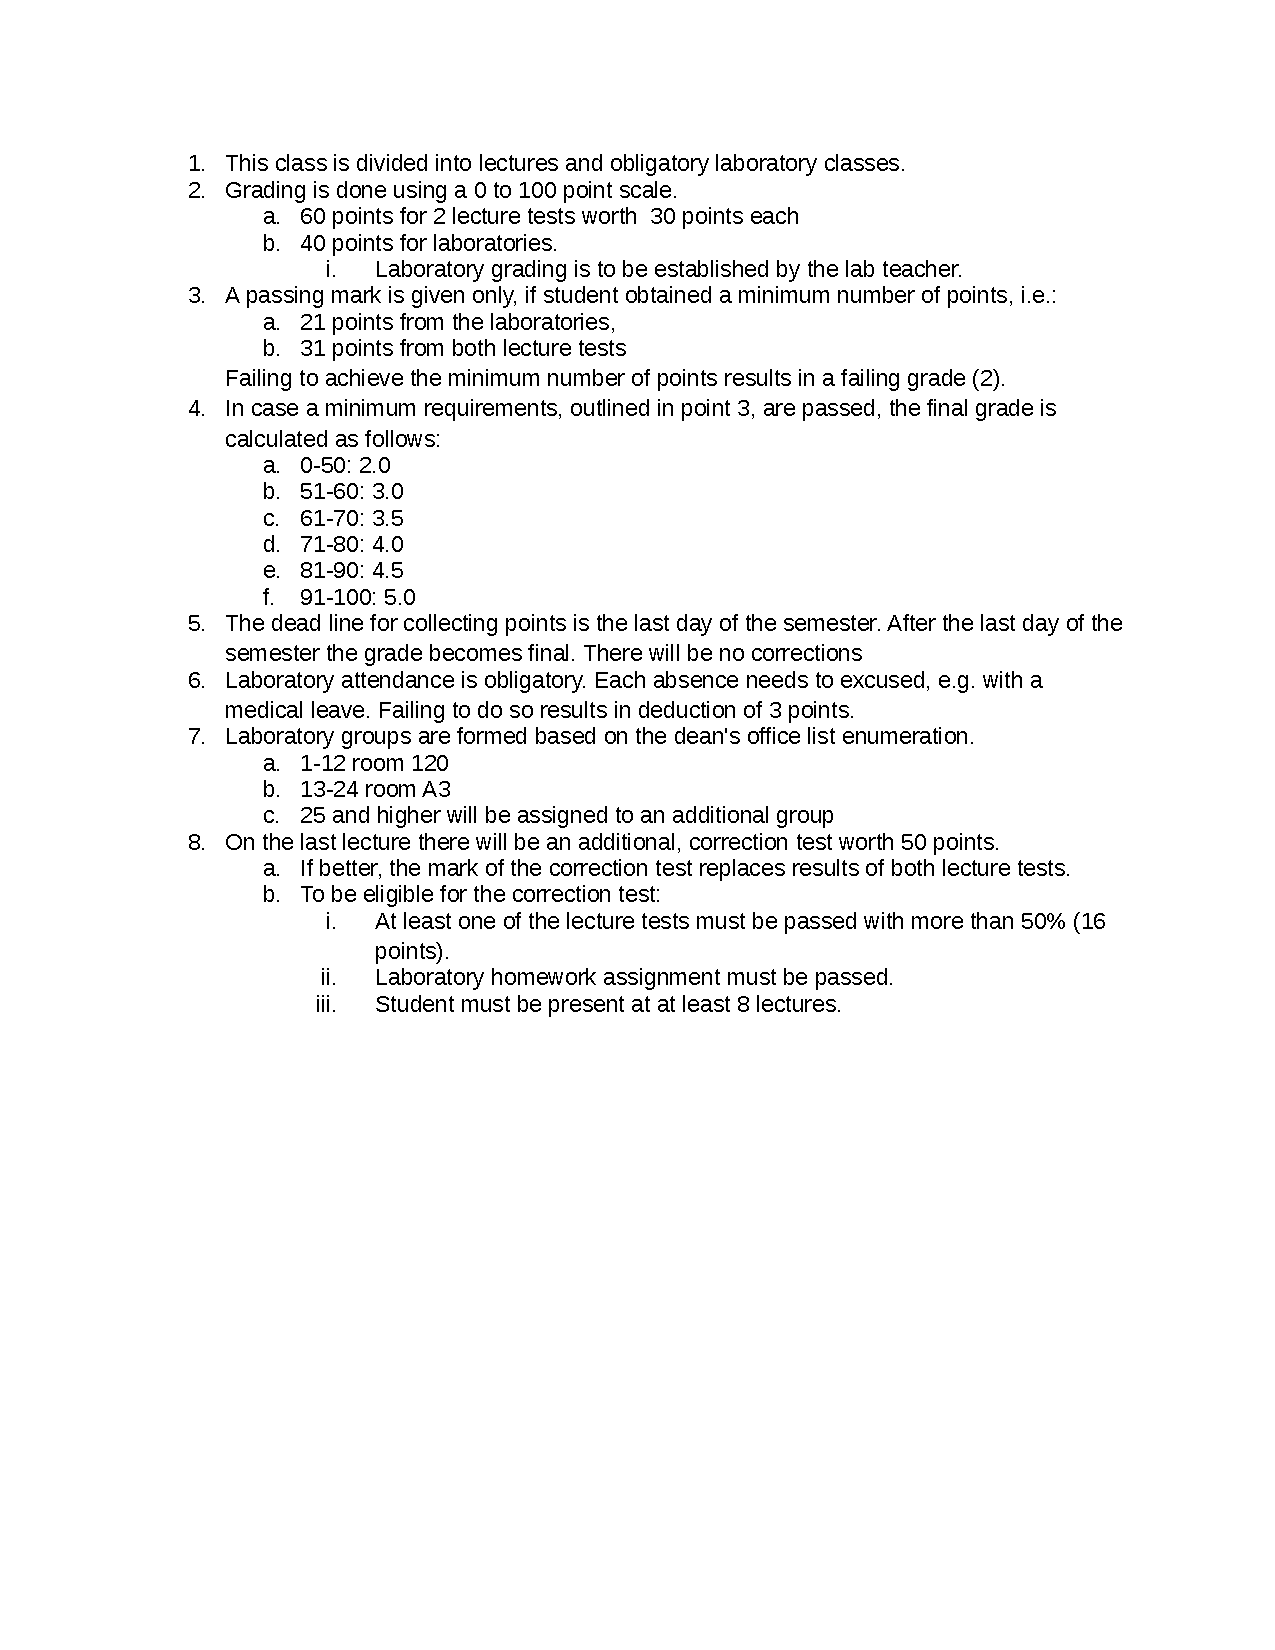
\includegraphics[height=\textheight, keepaspectratio, trim={3cm 9cm 3cm 2cm}, clip]{Rulesandregulations}
% }

\begin{frame}{Resources}
  \begin{itemize}
    \item Internet
    \item C / C++ programming tutorials
    \item Stack Overflow
    \item C / C++ reference online
    \item Google, Bing, Duck Duck Go ...
    \item Any Visual Studio or other IDE with C/C++ support
    \item It is like push-ups, you need practice, not books!
  \end{itemize}
\end{frame}

%%%%%%%%%%%%%%%%%%%%%%%%%%%%%%%%%%%%%%%%%%%%%%%%%%%%%%%%%%%%%%%%%%%%%%%
\section{Introduction}
%%%%%%%%%%%%%%%%%%%%%%%%%%%%%%%%%%%%%%%%%%%%%%%%%%%%%%%%%%%%%%%%%%%%%%%

\frame{
  \frametitle{Programming}
 
  \begin{columns}
    \begin{column}{0.49\textwidth}
      \begin{itemize}
        \item Act of writing instructions enabling the computer to perform desired tasks
        \item Ada Lovelace (1815 - 1852) - The first programmer    
      \end{itemize}
    \end{column}
    \begin{column}{0.49\textwidth}
      \centering
      \includegraphics[width=\textwidth, height=0.7\textheight, keepaspectratio]{Ada_Lovelace_portrait}\\
      {\tiny Source: Wikipedia, Science Museum / Science \& Society Picture Library}
    \end{column}
  \end{columns}
}

\frame{
  \frametitle{ C language}
    \begin{itemize}
      \item Dennis Ritchie – AT\&T Bell Laboratories - 1972
      \item The C Programming Language - first specification - 1978
      \item 1989: ANSI C89, 1990: ISO C90
      \item 1999: C99 standard
      \item Still in use, and here to stay for a while
      \begin{itemize}
        \item Wide range of applications. OS, microcontrollers, ATM systems ...
        \item Efficiency and performance
        \item Provides low level access
        \item Influenced C++, Obj. C, C\#, Java, ...
      \end{itemize}
    \end{itemize}
}

\section{First Program}

\begin{frame}[fragile]{First program}
      \begin{itemize}
        \item Text file with {\bf .c} extension (or .cpp ...)
        \item Edit with your favourite text editor (or an IDE)
        \item // this is a single line comment, this will not be processed
        \item /* this is a multi line comment, will not be processed */
      \end{itemize}

    \begin{lstlisting}
    /* Start with a short description of the program */
    #include <stdio.h> //Append the I/O library
   
    int main()
    {
      printf(" Hello students!! \n ");
    }
    \end{lstlisting}  
   
    \begin{itemize}
      \item \# lines starting with a hash are preprocesor directives. We will be seeing them.
      \item There has to be exactly one main function!
      \item Watch brackets!!
      \item (Almost) all instructions end with a semicolon ;
    \end{itemize}
   
\end{frame}

\begin{frame}[fragile]{Compile and Run}
\begin{lstlisting}[style=consol, numbers=none]
$ gcc hello.c
\end{lstlisting}
\centering
\includegraphics[width=0.7\textwidth, height=0.7\textheight, keepaspectratio]{GCC_CompilationProcess}
\newline In the end a.out
\vspace{0.2cm}

\begin{lstlisting}[style=consol, numbers=none]
$ gcc -Wall hello.c -o hello.out
\end{lstlisting}
Can get pretty long ...
\end{frame}

\section{Basic C elements}

\begin{frame}{Basic C elements}
  \framesubtitle{Allowable characters}
  \centering
  Characters we can use:
  \begin{itemize}
    \item a-z - lower case letters
    \item A-Z - upper case letters - different!
    \item 0-9 - digits
    \item (), [], \{\} - brackets
    \item +, -, *, /, \% - operations
    \item \, !, $<$, =, $>$
    \item \&, @, ., ,, :, ;, ', ", \#,
    \item And than some more!
  \end{itemize}
\end{frame}

\begin{frame}{Basic C elements}
  \framesubtitle{Keywords}
  \centering
  Reserved keywords that have a special meaning to the compiler:
  \vspace*{10pt}
  
  \begin{columns}
    \begin{column}{0.2\textwidth}
      auto\\
      breach\\
      case\\
      char\\
      const\\
      continue\\
      default\\
      do
    \end{column}
    \begin{column}{0.2\textwidth}
      double\\
      else\\
      enum\\
      extern\\
      float\\
      for\\
      goto\\
      if
    \end{column}
    \begin{column}{0.2\textwidth}
      int\\
      long\\
      register\\
      return\\
      short\\
      signed\\
      sizeof\\
      static
    \end{column}
    \begin{column}{0.2\textwidth}
      struct\\
      switch\\
      typedef\\
      union\\
      unsigned\\
      void\\
      volatile\\
      while
    \end{column}
  \end{columns}
 
\end{frame}

\begin{frame}{Basic C elements}
  \framesubtitle{User defined names}
  \centering
  As programmers we will need to give names to elements of our program:
  \vspace*{10pt}
  
  \begin{itemize}
    \item Functions, variables, constants (and some others) need an identifier
    \item Any sequence of letters, digits and an underscore can be a name
    \item First character must be a letter or an underscore
    \item An identifier can not be a keyword (see the previous slide)
    \item ax123(), x1(), dominateTheWorld(), RuleGalaxy111() are examples of admissible identifiers (names)
    \item Customary to start with a lower case letter
  \end{itemize}
\end{frame}

\section{Comments}

\begin{frame}[fragile]{Comments - ignored by the compiler}
    Use comments:
    \begin{itemize}
      \item to explain the code
      \item to describe what is done
      \item as notes
      \item for fun
    \end{itemize}
    \begin{lstlisting}
    /* This is a multi-line
       comment.
       It can go on
       through many lines until this: */
   
    // This is a single line comment, it stretches until the end of line. If there is no "new line" and the line is folded, it is still a single line.
   
    // sometimes I believe compiler ignores all my comments
    \end{lstlisting}
\end{frame}

\begin{frame}[fragile]{Comments Real life example}
  Comment found in one of the Stack Overflow as a warning ...
 
  \begin{lstlisting}
    //
    // Dear maintainer:
    //
    // Once you are done trying to 'optimize' this routine,
    // and have realized what a terrible mistake that was,
    // please increment the following counter as a warning
    // to the next guy:
    //
    // total_hours_wasted_here = 42
    //
  \end{lstlisting}
\end{frame}

\begin{frame}[fragile]{Program structure}

    \begin{lstlisting}
    /* Description - not mandatory but polite*/
    #include <stdio.h>
    #define PI 4.0*atan(1.0)
    \end{lstlisting}
    \vspace{0.2cm}

\end{frame}

\section{Program Structure}

\begin{frame}[fragile]{Program structure}
    \begin{lstlisting}
    /* Description - not mandatory but polite*/
    #include <stdio.h> //Preprocessor commands starting with a \#
    #define PI 4.0*atan(1.0) // Note no semicolons ";", why?
       
    int main()
    {
     
    }
       
    \end{lstlisting}
 
\end{frame}

\begin{frame}[fragile]{Program structure}
    \begin{lstlisting}
    /* Description - not mandatory but polite*/
    #include <stdio.h> //Preprocessor commands starting with a \#
    #define PI 4.0*atan(1.0) // Note no semicolons ";", why?
     
    int main() //The main function must be there
    { // <- the opening bracket
      // Body of a function, "the meat"
    } // <- The closing bracket
   
    // ==== Above obligatory, below additional user defined functions ====
   
    int sum_ints(int a, int b)
    {
      return a+b;
    }    
    \end{lstlisting}
 
\end{frame}

\begin{frame}[fragile]{Program structure}
    \begin{lstlisting}
    /* Description - not mandatory but polite*/
    #include <stdio.h> //Preprocessor commands starting with a \#
    #define PI 4.0*atan(1.0) // Note no semicolons ";", why?
   
    int sum_ints(int a, int b); //Function prototypes, a promise to the compiler
    int a=5; // Definition of global variables if needed. Not mandatory, more later.
   
    int main() //The main function must be there
    { // <- the opening bracket
      // Body of a function, "the meat"
    } // <- The closing bracket
   
    // ==== Above obligatory, below additional user defined functions ====
   
    int sum_ints(int a, int b)
    {
      return a+b;
    }
   
    ....
   
    \end{lstlisting}
 
\end{frame}

\begin{frame}[fragile]{Headers}

    \begin{lstlisting}
    /* Description - not mandatory but polite*/
    #include <stdio.h>
    #include "myheader.h"
    \end{lstlisting}
    \vspace{0.2cm}

  \begin{itemize}
    \item Header files contain constants, functions, other declarations
    \item System or user generated
    \item \#include $<$stdio.h$>$ - read the contents of the header file stdio.h
    \item stdio.h: standard input/output for console and files
    \item \#include $<$stdio.h$>$ - look for system headers
    \item \#include "mygreatheader.h" - look for user generated headers in ./
  \end{itemize}
 
\end{frame}

\begin{frame}[fragile]{Functions}

    \begin{lstlisting}

    int sum_ints(int a, int b); //A prototype end with semicolon

    //type name (arguments)
    int main(void)// main can have arguments
    {
      return 0; // main is special!
    }
   
    //this function is of integer type
    int sum_ints(int a, int b) //it accepts two arguments of integer type
    {
      return a+b; // since it has a type it must have a return.
    }
    \end{lstlisting}
    \vspace{0.2cm}
 
\end{frame}






\end{document}
